% This is samplepaper.tex, a sample chapter demonstrating the
% LLNCS macro package for Springer Computer Science proceedings;
% Version 2.20 of 2017/10/04
%
\documentclass[runningheads]{llncs}
%
\newcommand{\todo}[1]{\textbf{\textcolor{red}{TODO: #1}}} 

\usepackage{graphicx}

\usepackage{cite}
\usepackage{amsmath,amssymb,amsfonts}
\usepackage{algorithmic}
\usepackage{graphicx}
\usepackage{textcomp}
\usepackage{xspace}
\usepackage{url}
\def\BibTeX{{\rm B\kern-.05em{\sc i\kern-.025em b}\kern-.08em 
    T\kern-.1667em\lower.7ex\hbox{E}\kern-.125emX}}
    
% Put edit comments in a really ugly standout display
\usepackage{times}
 
% Macros for proof-reading & corrections
\usepackage[normalem]{ulem} % for \sout  
\usepackage{xcolor} 

% Macros for proof-reading & corrections
\usepackage[normalem]{ulem} % for \sout  
\usepackage{xcolor} 

\usepackage{ifthen}
\usepackage{amssymb} 
\newboolean{showcomments}  
\setboolean{showcomments}{true} % toggle to show or hide comments
\ifthenelse{\boolean{showcomments}}     
  {\newcommand{\nb}[2]{
    \fcolorbox{gray}{yellow}{\bfseries\sffamily\scriptsize#1}
    {$\blacktriangleright$#2$\blacktriangleleft$}
   }
   \newcommand{\version}{\emph{\scriptsize$-$working$-$}} 
  }
  {\newcommand{\nb}[2]{}
   \newcommand{\version}{} 
  } 

\newcommand\levi[1]{\nb{Levi}{\textcolor{teal}{#1}}}
\newcommand\hernan[1]{\nb{Hernan}{\textcolor{teal}{#1}}}

\newcommand{\af}{\textsc{AF3}\xspace}
\newcommand{\autofocus}{\textsc{AutoFOCUS3}\xspace}

% Used for displaying a sample figure. If possible, figure files should
% be included in EPS format.
%
% If you use the hyperref package, please uncomment the following line
% to display URLs in blue roman font according to Springer's eBook style:
% \renewcommand\UrlFont{\color{blue}\rmfamily}

\begin{document}
%
\title{Controlling a Virtual Rover using AutoFOCUS3}
%
%\titlerunning{Abbreviated paper title}
% If the paper title is too long for the running head, you can set
% an abbreviated paper title here
%
\author{Levi L\'ucio \and
Sudeep Kanaav} 
%
\authorrunning{Levi L\'ucio and Sudeep Kanaav}
% First names are abbreviated in the running head.
% If there are more than two authors, 'et al.' is used.
%
\institute{fortiss GmbH\\ Guerickestra\ss e 25\\80805 M\"unchen\\
\email{\{lucio,kanav\}@fortiss.org}}
%
\maketitle              % typeset the header of the contribution
%
\begin{abstract}
\autofocus (\af) is a mature model-driven engineering environment to develop
software for embedded systems. For the past 20 years, several versions of \af
have served as a platform for experimenting with cutting edge research ideas in
Model-Driven Development.
\af is a tool that fully encompasses the software lifecycle, from requirements,
to architecture, simulation, deployment, code generation and verification. The
attendees of this tutorial will be given the unique opportunity to model and deploy
software on a real remote-controlled vehicle, using only \af.\levi{finish this
abstract}
 
\keywords{First keyword  \and Second keyword \and Another keyword.}
\end{abstract}
  
\section{Introduction}

\autofocus is a model-based development (MBD) environment for embedded systems,
based on the \textsf{Focus} theory~\cite{Broy:2001:SDI:374869}. \textsf{Focus} is a framework
encompassing computations supported by the notion of streams (“in particular
untimed, timed and time-synchronous streams”
\cite{Holzl:2007:AST:1927558.1927576}). The current version of \af follows a
string of earlier
prototypes~\cite{Holzl:2007:AST:1927558.1927576,DBLP:conf/models/AravantinosVTHS15}
started in 1996~\cite{Huber96autofocus--}. Existing literature on \af (some of
it published at MODELS) reports on particular aspects of the
tool~\cite{TMR2013,TMR2011,Lucio:17,DBLP:conf/se/VossEH14,Barner2016,Diewald2016,Carlan2017},
or on its application in the context of industrial case
studies~\cite{2009-a-top-down-methodology-for-the-development-of-automotive-software,2011KeylessEntry,Bohm:2014:FSE:2593850.2593856,DBLP:conf/models/AravantinosVTHS15,Barner2017,Eder2017}.
More information about current state of the \af-related research can be found in
the official site of the tool\footnote{ https://af3.fortiss.org/}. \af can be
freely downloaded and is open-source.

\af's goal is to demonstrate the feasibility and applicability of
MBD tooling approaches. The idea behind \af embraces seamless integration of all models throughout the
development process, encompassing requirements engineering on initial stage, system
modeling at a high level of abstraction, deployment and model simulation. \af
also comprises formal verification and testing. Being an open source tool with a 6 months
release period, \af embodies a study tool for proving scientific concepts and
methods which have been tested via industrial case studies.

In the context of domain-specific development, there are several approaches to
system modeling. The first of those is characterized by starting from a general
(non platform-specific) model and proceed by transforming this model into
specialized one. In this approach, domain specific languages are built by
restricting a universal language (such as the UML) and incarnated as development
tools. This is the “Model-Driven Architecture” concept and is represented by
such tools as Enterprise Architect~\cite{SparxSystems} or
Papyrus~\cite{Papyrus}. \af embodies a “bottom-up” approach, which aims at
guiding the modeler until full creation of domain-specific model.
In comparison with the former approach, \af follows the domain-specific modeling
philosophy, where only the strictly required concepts are developed into tools while starting
from a blank slate. The goal is to minimize the possibility of error by
enforcing, as much as possible, correctness-by-construction. Additionally, \af
is built on top of an extensible kernel which constitutes a base for further
development. Examples of other tools that follow \af's ``bottom-up'' approach are
Sirius\cite{Sirius} or JetBrains' MPS\cite{MPS}.

Tools that resemble \af in some way are Enterprise
Architect~\cite{SparxSystems}, Papyrus~\cite{Papyrus}, UML Designer~\cite{UMLDesigner}, Sirius\cite{Sirius}, JetBrains' MPS~\cite{MPS},
mbeddr~\cite{mbeddr} or Simulink~\cite{simulink}. Although space does not allow elaborating on the
differences between these tools and \af, our tool is to the best of our knowledge the
only open-source model-driven tool that supports the whole embedded-software development
cycle in an out-of-the-box, easily installable package. \af includes support
for requirements engineering, formal verification, deployment or domain space
exploration cases natively (among other features), which we have not found in
combined in one unique package in other tools.\\

In this paper we explain how we have developed an \af model to operate a rover
in a virtual environment in a way that it follows another leader rover that
advances freely, while always keeping a safe distance. ``Sensor" data regarding
the position of the rover in front and the distance between the two rovers is
provided by the environment. The rover has access to its own position and angle
of movement and should constantly adjust its speed and angle by directing power
to the wheels (turning implies asymetrically providing power to the left and
right wheels). The virtual environment the rover functions on has been proposed
is part of the MDE tool challenge proposed by the MDE Tools workshop at the
MODELS 2018 conference.

The paper is organized as follows. In \sect\ref{sec:toy_rover_controller} we
provide a high level description of a controller built in \af for a physical car in the
context of a lab course offered at the Technical University of Munich.
Section~\ref {sec:control_vr_model} then describes how we have adapted the
Adaptive Cruise Control component built during the lab courses to serve the
purpose of following the leader. In \sect\ref{sec:deploy_generate} we explain
how we have deployed the model and generated \clang code for the controller. Section
\sect\ref{sec:conclusion} concludes.


\section{Control a Physical Toy Rover with AutoFOCUS3}

\section{Controlling the Virtual Rover}

In \fig\ref{fig:acc_model} we depict the top-level model of the controller for
follower vehicle. The controller is meant to function in a loop by reading the
\emph{Velocity} of the follower rover itself, the velocity of the leader rover
(input by the \emph{VelocityFrontObstacle} signal) and the \emph{distance} to
the leader rover. By using these values it constantly updates the maximal
allowed acceleration (\emph{MaxAcceleration}) as well as
the target velocity (\emph{TargetVelocity}) for the follower rover.

The controller is composed by a number of \af components, as follows:
\begin{itemize}
  \item the \emph{TargetDistance} component is responsible for calculating the ideal
distance to the leader rover. This distance is proportional to the speed of
the leader, as larger speeds imply larger distances for breaking. 
  \item The \emph{P Controller} component is a PID controller for adjusting the
the velocity of the follower in order to reach the target distance to the
leader.
\item The \emph{TargetVelocityController} component decides whether the
\emph{TargetVelocity} output should remain the same as in the previous step
(saved in the \emph{MaxVelocityMemory}) or should be updated to the
\emph{TargetVelocityIn} calculated by the \emph{P Controller} component.
\levi{don't understand this part of the model}
\end{itemize}


\begin{figure}[!h]
\centering
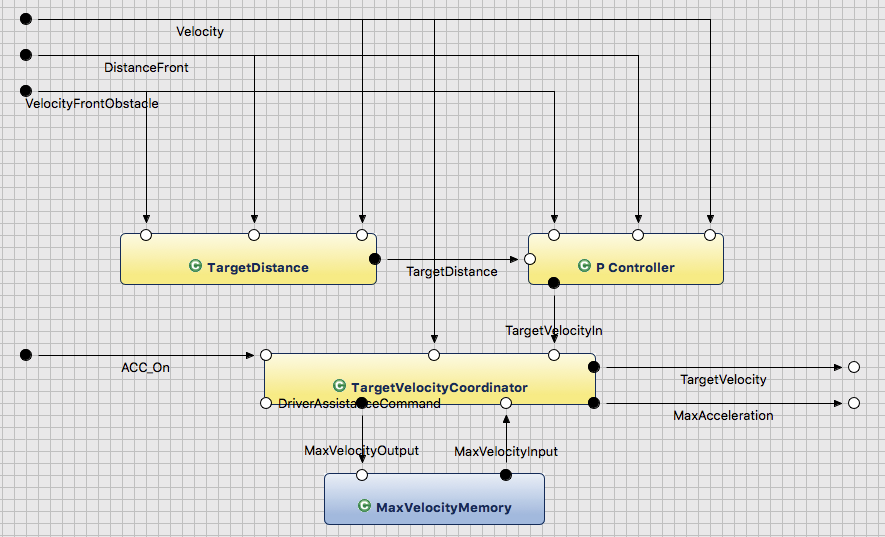
\includegraphics[width=1\textwidth]{images/ACC_controller_model.png}
\caption{The controller for the Automatic Cruise Control modelled in \af}
\label{fig:acc_model}
\end{figure}

\begin{figure}[!h]
\centering
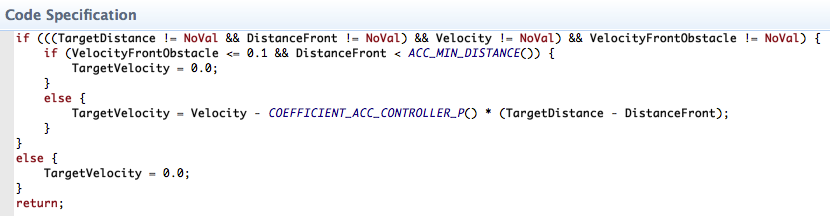
\includegraphics[width=1\textwidth]{images/code_spec_P_controller.png}
\caption{PID controller \af}
\label{fig:pid_controller}
\end{figure}

\begin{figure}[!h]
\centering
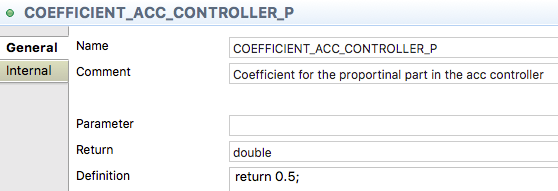
\includegraphics[width=.7\textwidth]{images/P_coefficient_controller.png}
\caption{P Coefficient}
\label{fig:p_coefficient}
\end{figure}  

\section{The Deployment Model}

\section{Deployment and Code Generation}
\label{sec:deploy_generate}

After the model is built, it needs to be deployed on an architecture. For the
real rover mentioned in \sect~\ref{sec:toy_rover_controller} the architecture
is a Raspberry Pi that can connect to the sensors and actuators of the device.

The virtual rover simulation environment used in the context of this article
communicates using TCP ports. Additionally, the signals flowing from the virtual
environment and back are different from the ones for the real rover. For
instance, the real rover accepts \emph{target speed} as input and the hardware
of the rover itself controls engine power (using an embedded \pid controller) in
order to attain such a speed and maintain it. The virtual rover expects that
power to the wheels is provided as a means to attain a certain speed.

\af provides a generic, non-device specific architecture for deployment, as
shown in \fig~\ref{fig:deployment_general}.

\begin{figure}[!h]
\centering
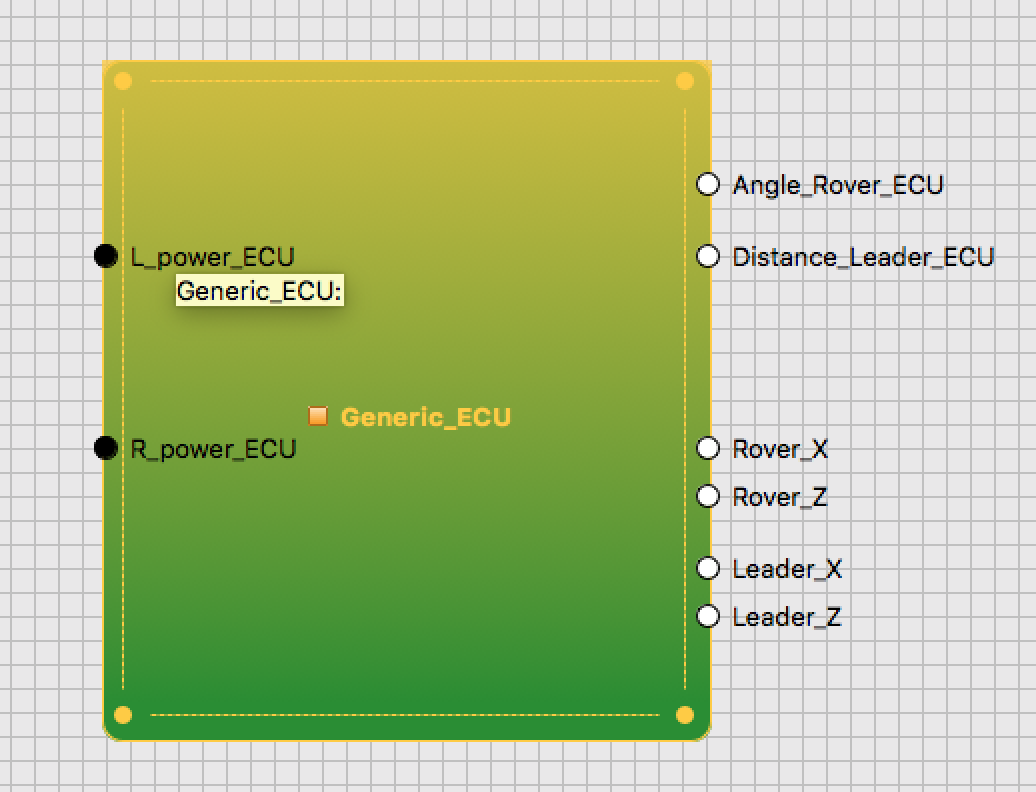
\includegraphics[width=.8\textwidth]{images/newECU.png}
\caption{A Generic ECU for the Virtual Rover Controller}
\label{fig:deployment_general}
\end{figure}

Additionally, the ports of the of the \ecu need to be mapped to the logical
ports of the controller of the model we have defined in
\sect~\ref{sec:control_vr_model}, as depicted in
figure~\ref{fig:deployment_ports}.

\begin{figure}[!h]
\centering
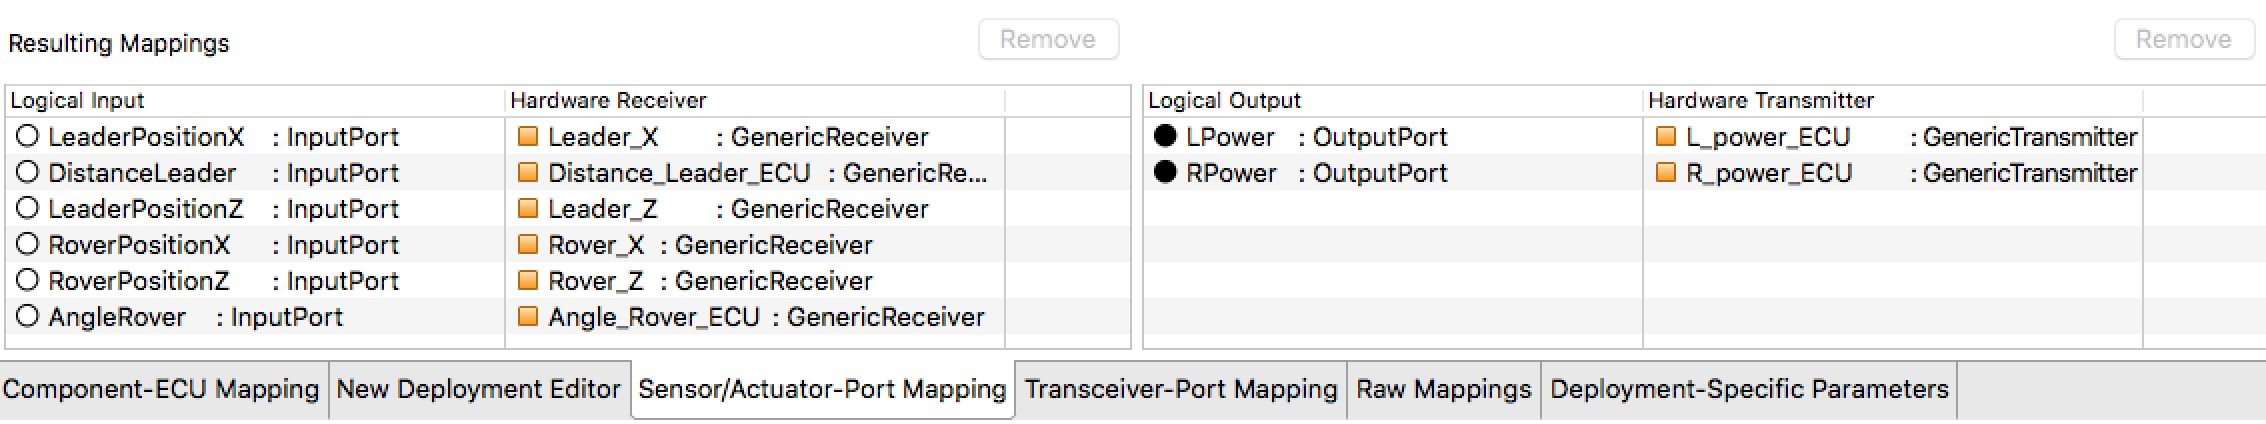
\includegraphics[width=1\textwidth]{images/newMapping.png}
\caption{Deploying the Logical Ports onto the \ecu ports}
\label{fig:deployment_ports}
\end{figure}
 
Deploying to an architecture provides the skeleton of an interface that declares
the signatures of the methods that are used by the controller logic to
communicate with the device underneath. When the architecture is fully defined,
then the glue code with the device can also be automatically generated. For our
work we have deployed onto a generic architecture as a means to automatically
generate the structure of our controller's communication infrastructure as \clang\footnote{Besides \clang, \af also allows the generating \java code.} code. The logic corresponding to the model we have presented in
\sect~\ref{sec:toy_rover_controller} is also generated as \clang code and is
meant to run in a loop with the controlled device, in this case the virtual
rover.

The \clang code that is generated for the generic architecture only provides the
interface for the functions that read the sensors and send commands on the
actuators of the virtual environment. Because of that, a manual step of
coding such methods and connecting the controller with the virtual environment
via TCP was additionally necessary to connect the controller to the rover and to
finalize the deployment of the model onto the hardware.




\section{Connecting to the Virtual Environment}
\label{sec:connect_virtual_env}

The logic of the controller for the rover that us generated in \clang can then
run in an infinite loop, cycling over reading the inputs from the sensors in the
rover and then computing and sending values to its actuators. The \clang
code that is generated for the generic architecture only provides the
interface for the functions that read the sensors and send commmands on the
actuators of the virtual environment. Because of that, a manual step of
coding such methods and connecting the controller with the virtual environment
via TCP was additionally necessary to connect the controller to the rover. 


\section{Running the Model in the Simulated Environment}

\section{Conclusion}
\label{sec:conclusion}

We have presented in this article the lifecycle of the development of
a controller for a virtual rover, based on a controller for a real vehicle
developed at lab courses given by us. Our experience points to the fact that \af is
a sufficiently mature environment for developing embedded systems, in
particular controllers. The facilities for generating code for a specific platform (in our case a generic one) make life
for the developer of embedded code simple, as the communication infrastructure
with the underlying hardware can be fully automated. We have observed this
advantage when we, in the course of the lab courses, deployed the code
generated from models directly to Raspberry Pis, without any need for further customization. Additionally, the modularity enforced by \af
makes it easy to reuse parts of projects. We found that the copy/paste
facilities of \af are very helpful in that respect.

We have certainly encountered editing issues with \af's editor while building
the model for the challenge, but they were minor and the modelling experience
was very slighted affected by them. The calibration of controllers such as the
one we present in this paper also poses a problem, as it is mostly only
possible once the hardware is in the loop with the generated code. \af does not
provide a basic infrastructure for calibration (although a prototypical version
of such an infrastructure does exist). In practice, we have observed that a
significant amount of time still needs to be devoted to making sure the
parameters of the controller are well configured.
 

\bibliographystyle{abbrv} 
\bibliography{./references}

\end{document}
